\classheader{2018-08-22}
For $\vec{x}' = A_{2x2}\vec{x}$,
\begin{enumerate}[label=\protect\circled{\Roman*}]
	\item One can construct a slope field in $\mathbb{R}^2$ via matrix multiplication: For $\vec{x} \in \mathbb{R}^2$, the tangent to the solution curve passing through is $\vec{x} = \begin{bmatrix}
		x_1\\ x_2
	\end{bmatrix}$ is $A\vec{x}$
	\begin{enumerate}[label=\protect\circled{\alph*}]
		\item $\vec{x} = \begin{bmatrix}
			1\\2
		\end{bmatrix}$, $\vec{x} = \begin{bmatrix}
			1 & 1\\ 6 & 0
		\end{bmatrix}
		\begin{bmatrix}
			1\\2
		\end{bmatrix} = 
		\begin{bmatrix}
			3\\6
		\end{bmatrix}$
		\item $\vec{x} = \begin{bmatrix}
			1\\0
		\end{bmatrix}$, $\vec{x} = \begin{bmatrix}
			1 & 1\\ 6 & 0
		\end{bmatrix}
		\begin{bmatrix}
			1\\0
		\end{bmatrix} = 
		\begin{bmatrix}
			1\\6
		\end{bmatrix}$
		\item $\vec{x} = \begin{bmatrix}
			0\\1
		\end{bmatrix}$, $\vec{x} = \begin{bmatrix}
			1 & 1\\ 6 & 0
		\end{bmatrix}
		\begin{bmatrix}
			0\\1
		\end{bmatrix} = 
		\begin{bmatrix}
			1\\0
		\end{bmatrix}$
	\end{enumerate}
	JODE 2D calculator or similar is helpful here.
	\item Solution curves are integral curves of the slope field:
	\begin{enumerate}[label=\protect\circled{\alph*}]
	\item Given $c_1, c_2 \in \mathbb{R}$, the curve $\vec{x(t)} = c_1 \begin{bmatrix}
				1\\2
			\end{bmatrix} e^{3t} + c_2
			\begin{bmatrix}
				1\\-3
			\end{bmatrix} e^{-2t}$ is one of these curves.
	\item Straight line motion only occurs when $c_1 = -2, c_2 = 0$. Then $\vec{x}(t) = -2 \begin{bmatrix}
	1\\2
\end{bmatrix} e^{3t} = \begin{bmatrix}
	-2\\-4
\end{bmatrix}e^{3t}$
	\item A copy of $\mathbb{R}^2$ with enough representative curve on it to give a sound sense of solutions is called a \underline{phase portrait}.
	\item Solutions are called \underline{trajectories} or \underline{orbits}.
	\item General long term behaviour of trajectories can be read off easily from a phase portrait:
	\begin{equation*}
		\text{Given } \quad \vec{x}(t) = c_1 \begin{bmatrix}
				1\\2
			\end{bmatrix} e^{3t} + c_2
			\begin{bmatrix}
				1\\-3
			\end{bmatrix} e^{-2t},
	\end{equation*}
	\begin{itemize}
		\item If $c_1 = 0$, $c_2 \neq 0$, then $\vec{x}(t) = c_2
			\begin{bmatrix}
				1\\-3
			\end{bmatrix} e^{-2t}$ and $\vec{x}(t) = c_2
			\begin{bmatrix}
				1\\-3
			\end{bmatrix} e^{-2t}$ and $\Lim{t \rightarrow \infty} \vec{x}(t) = \begin{bmatrix}
				0\\0
			\end{bmatrix}$ How about $\Lim{t \rightarrow -\infty} \vec{x}(t)?$ We say it is \underline{unbounded}.\\
		\textbf{Note: } Solutions never touch nor cross here. So since $\vec{x}(t) = \begin{bmatrix}
				0\\0
			\end{bmatrix}$ is in equilibrium solution, no other solution actually reader $\begin{bmatrix}
				0\\0
			\end{bmatrix}$
		\item If $c_1 \neq 0, c_2 = 0$?\\
		$\Lim{t \rightarrow \infty} \vec{x}(t)$ DNE on trig is unbounded\\
		$\Lim{t \rightarrow -\infty} \vec{x}(t) = \begin{bmatrix}
			0\\0
		\end{bmatrix}$
		\item If $c_1 \neq 0$ and $c_2 \neq 0$? These are the curved lines in the portrait. For these, what can we say about the forward trajectory ($\Lim{t \rightarrow \infty} \vec{x}(t)$), or the backward one ($\Lim{t \rightarrow -\infty} \vec{x}(t)$)?\\
		One Answer? Given $\quad \vec{x}(t) = c_1 \begin{bmatrix}
				1\\2
			\end{bmatrix} e^{3t} + c_2
			\begin{bmatrix}
				1\\-3
			\end{bmatrix} e^{-2t}$ and $c_1 \neq 0$, $c_2 \neq 0$, then as $t$ gets large $(t \rightarrow \infty)$, $\vec{x}(t)$ looks more and more like $c_1 \begin{bmatrix}
				1\\2
			\end{bmatrix} e^{3t}$, and less and less like $c_2
			\begin{bmatrix}
				1\\-3
			\end{bmatrix} e^{-2t}$. How about in backward time?
	\end{itemize}
	\begin{center}
		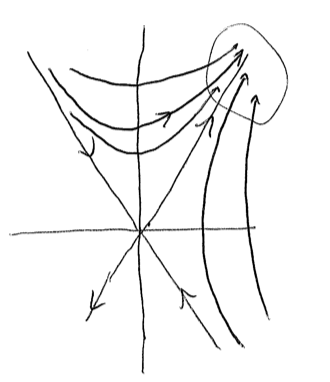
\includegraphics{23-1}
	\end{center}
	\end{enumerate}
	\item Back to solution building via properties of A: For $\vec{x} = \begin{bmatrix}
			1 & 1\\ 6 & 0
		\end{bmatrix} \vec{x}$, 
		\begin{equation*}
			\vec{x}(t) = c_1 \begin{bmatrix}
				1\\2
			\end{bmatrix} e^{3t} + c_2
			\begin{bmatrix}
				1\\-3
			\end{bmatrix} e^{-2t}
		\end{equation*}
		the eigenvalues of A ($\Gamma_1 = 3, \Gamma_2 = -2$), and representive eigenvectors ($\vec{v_1} = \begin{bmatrix}
			1\\2
		\end{bmatrix}, \vec{v_2} = \begin{bmatrix}
			1\\-3
		\end{bmatrix}$) are explicitly part of the solution. \underline{Why?}\\
		Here, the eigenvalues and eigenvectors of a matrix $A$ satisfy $A\vec{v} = \lambda \vec{v}$, or $(A - \lambda I)\vec{v} = \vec{0}$\\
		For this to have non trivial solutions for $\vec{v}$,
		\begin{itemize}
			\item $\lambda$ must be an eigenvalue, and 
			\item $\det (A - \lambda I) \vec{v} = \vec{0}$
		\end{itemize}
		For $A = \begin{bmatrix}
			a& b\\ c& d
		\end{bmatrix}, \det (A- \lambda I) = \begin{vmatrix}
			a - \lambda & b\\
			c & d - \lambda
		\end{vmatrix} = 0$\\
		$ = \lambda^2 - (a + d)\lambda + (ad - bc) = 0$\\
		This is called the \underline{characteristic equation} of A, and solutions can be
		\begin{enumerate}[label=\protect\circled{\arabic*}]
		\item real, distinct
		\item real and repeated
		\item complex conjugates
		\end{enumerate}
		How to relate to solutions of $\vec{x}' = A\vec{x}$?
		\begin{itemize}
			\item Recall $\dot{x} = ax$ is solved by $x(t) = ce^{at}$
			\item Assume $\dot{\vec{x}} = A\vec{x}$ is also solved by exponentials. For $n=2$, $\vec{x} = \begin{bmatrix}
				x_1 \\x_2
			\end{bmatrix}$. Assume $x_1(t) = c_1e^{\Gamma t}$, $x_2(t) = c_2e^{\Gamma t}$\\
			$\Rightarrow \vec{x}(t) = \begin{bmatrix}
				c_1\\c_2
			\end{bmatrix} e^{\Gamma t}$, and $\vec{x}' = \Gamma \begin{bmatrix}
				c_1\\c_2
			\end{bmatrix} e^{\Gamma t}$ and then $\vec{x}' = A \vec{x}$ is $\Gamma \begin{bmatrix}
				c_1\\c_2
			\end{bmatrix} e^{\Gamma t} = A \begin{bmatrix}
				c_1\\c_2
			\end{bmatrix} e^{\Gamma t}$ or $\Gamma \begin{bmatrix}
				c_1\\c_2
			\end{bmatrix}  = A \begin{bmatrix}
				c_1\\c_2
			\end{bmatrix}$, is $\Gamma \vec{v} = A\vec{v}$.\\
			And what do solutions to this look like? 
			\begin{itemize}
			\item $\Gamma$ is an eigenvalue
			\item $\vec{v}$ is an eigenvector of $\Gamma$.
			\end{itemize}
		\end{itemize}
		\textbf{Notes: }
		\begin{enumerate}[label=\protect\circled{\arabic*}]
		\item This works equally well for $n > 2$.
		\item In the case where $A_{nxn}$ is real and symmetric (i.e. when $a_{ij} = a_{ji}$)\\
		$\Rightarrow$ all eigenvalues one real and even if repeated, there is a full set of eigenvectors.
		\end{enumerate}
		We have the following:\\
		For $\dot{\vec{x}} = A_{nxn} \vec{x}$, when all eigenvalues of A are real and distinct, then
		\begin{equation*}
			\vec{x}(t) = c_1\vec{v_1}e^{\Gamma_1 t} + \cdots + c_n\vec{v_n}e^{\Gamma_n t}
		\end{equation*}
		is the general solution, where $\vec{v_i}$ is on eigenvector of $\Gamma_i$ for A.
\end{enumerate}